
\subsubsection{World One}

In extracting this World we decided to concentrate on a single user reality, in order to make it simpler to understand the usage of the application within the User context.
\\As you can easily see, what this diagram shows is the \textbf{Meeting} entity and the relationships it has with the \textbf{Travels}, the \textbf{Warnings} and the \textbf{Locations}.
\\Having a lot of meetings for a single user allows us to raise the probabilities to have conflicts between meetings, this is mainly because conflicts have to be in the same calendar (thus they have to be of the same User).
\\You can notice there are two Warnings, only connecting meetings with the \textbf{WithWarning status}, all meetings belonging to the warning are related to the each other and are connected to the warning, you can also see that there cannot exist two meetings in conflict with each other of which the appointment location is the same (obviously because if the user is already at the appointment site he cannot be late for the next meeting.
\\Another things to notice is that a meeting scheduled in a time where the weather forecast says it's going to rain, (\textbf{weather : Rainy}, where rainy symbolizes any type of 'bad weather') cannot have a \textbf{route} which involves the usage of means of transport where the user could wet himself (Bike, SharedBike, OnFoot).

\begin{figure} 

\begin{center}

\makebox[\textwidth]{%
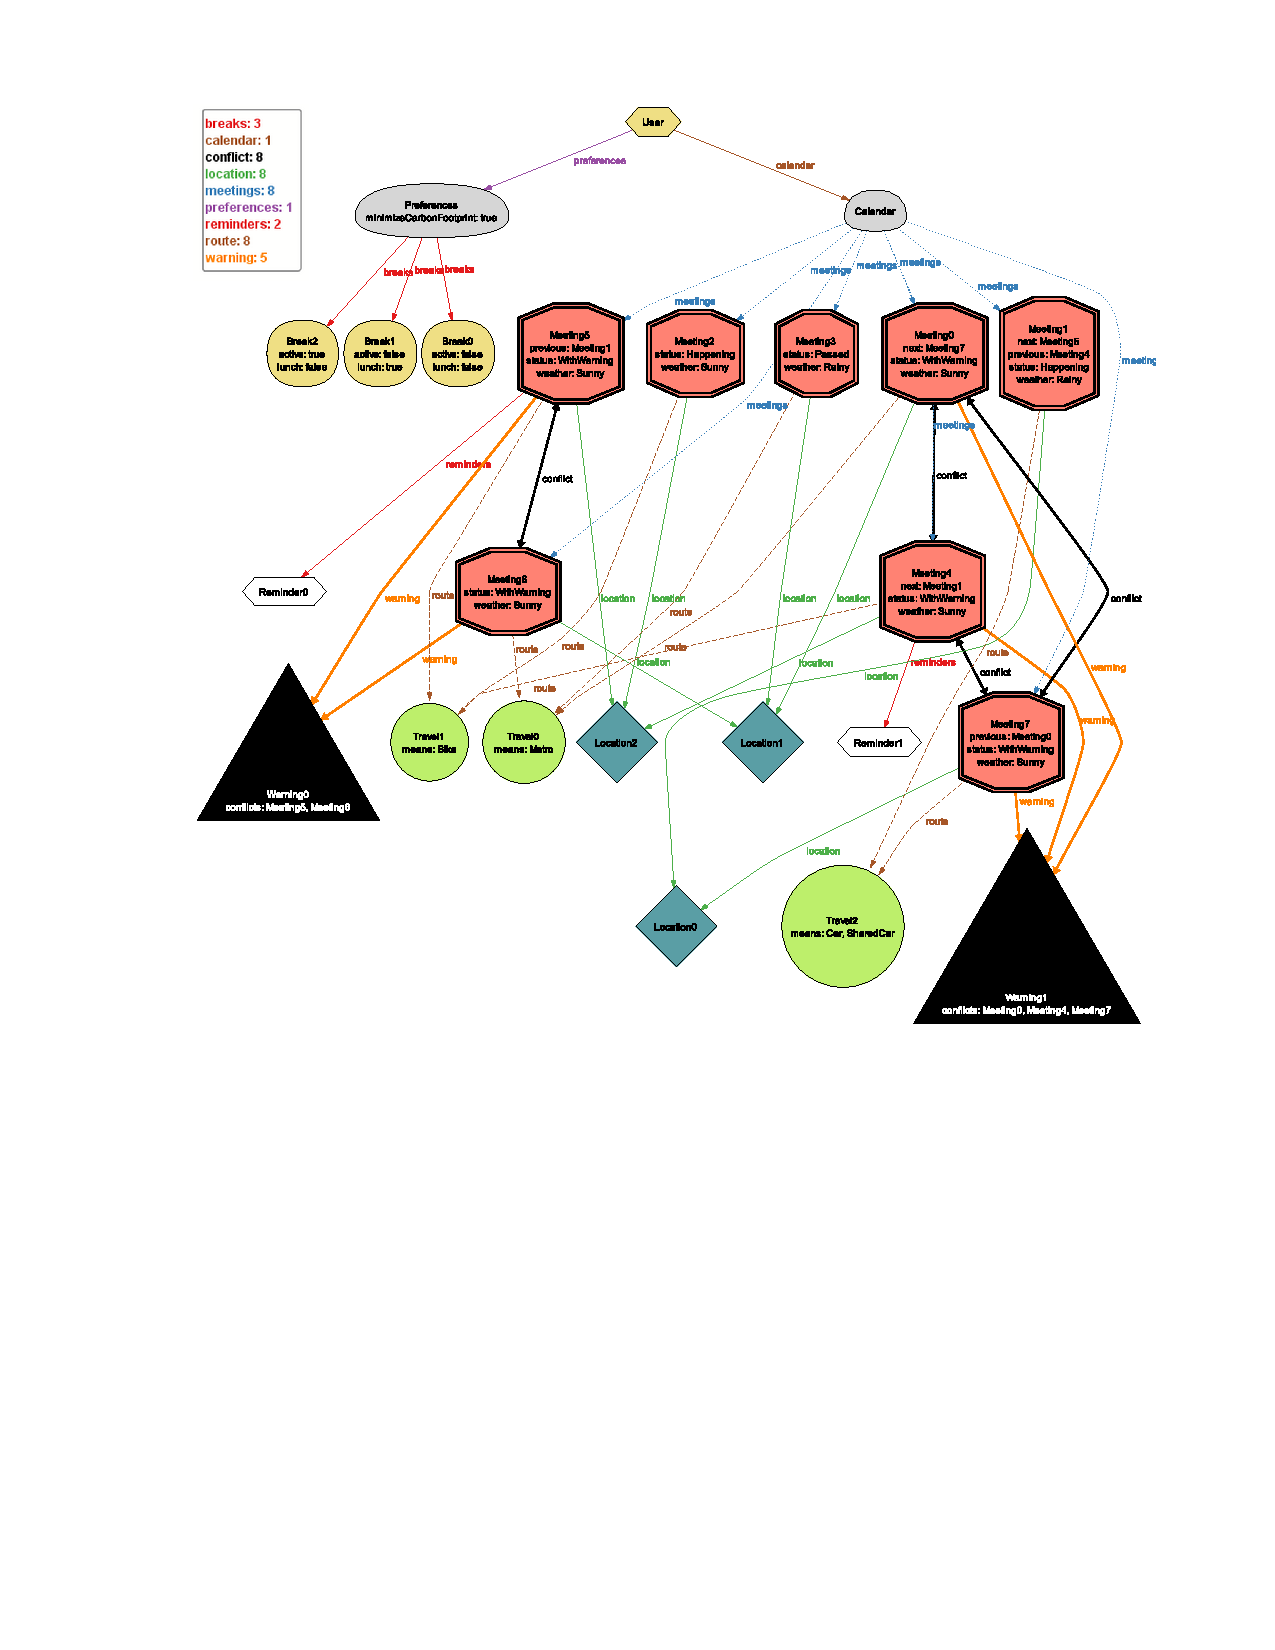
\includegraphics[width=1.7\linewidth]{alloy/world1pdf} 
}
\caption{Alloy World 1} 
\label{fig:alloyworld1} 


\end{center}
\end{figure} 

\clearpage
\subsubsection{World Two}

The second world was extracted in such a way that allow us to look for irregularities at the multi-client application, hence looking at consistency from the server-side.
\\We specified we wanted to have more than one User in order to be able to understand if the various meetings would not mix up neither between calendar nor between users.
\\An important thing that can be shown from this diagram is that the only warning is generated between two meetings belonging to the same Calendar (thus they are of the same User), and of course as we have seen in the previous world there cannot be meetings in conflict with each other if they are pointing at the same location.
\\The last thing to notice is that the Time relation symbolized by the previous relation and next relation works just fine, the next relation is the defined as the transposition of previous.


\begin{figure} 

\begin{center}

\makebox[\textwidth]{%
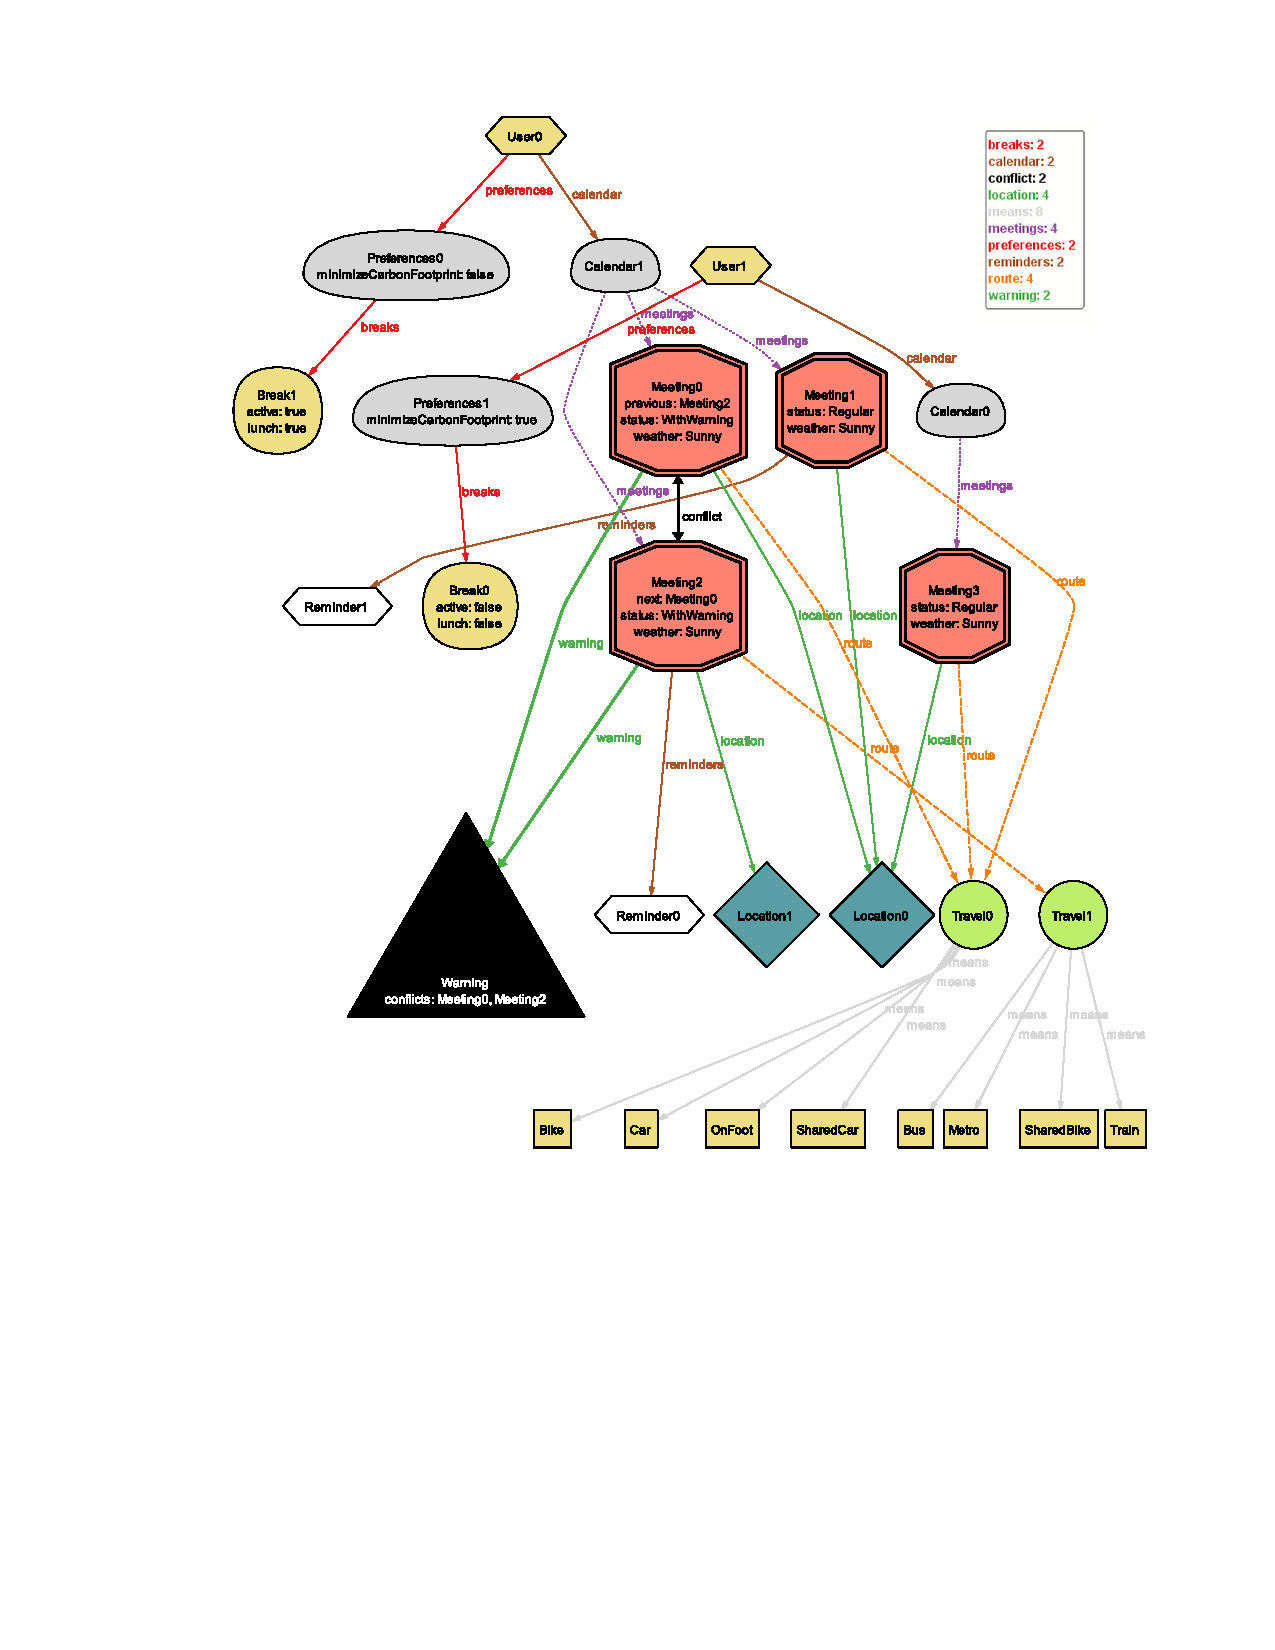
\includegraphics[width=1.6\linewidth]{alloy/world2pdf} 
}
\caption{Alloy World 2} 
\label{fig:alloyworld2} 


\end{center}
\end{figure} 

